\documentclass[letter, 11pt]{article}
%% ================================
%% Packages =======================
\usepackage[utf8]{inputenc}      %%
\usepackage[T1]{fontenc}         %%
\usepackage{lmodern}             %%
\usepackage[spanish]{babel}      %%
\decimalpoint                    %%
\usepackage{fullpage}            %%
\usepackage{fancyhdr}            %%
\usepackage{graphicx}            %%
\usepackage{amsmath}             %%
\usepackage{color}               %%
\usepackage{mdframed}            %%
\usepackage[colorlinks]{hyperref}%%
%% ================================
%% ================================

%% ================================
%% Page size/borders config =======
\setlength{\oddsidemargin}{0in}  %%
\setlength{\evensidemargin}{0in} %%
\setlength{\marginparwidth}{0in} %%
\setlength{\marginparsep}{0in}   %%
\setlength{\voffset}{-0.5in}     %%
\setlength{\hoffset}{0in}        %%
\setlength{\topmargin}{0in}      %%
\setlength{\headheight}{54pt}    %%
\setlength{\headsep}{1em}        %%
\setlength{\textheight}{8.5in}   %%
\setlength{\footskip}{0.5in}     %%
%% ================================
%% ================================

%% =============================================================
%% Headers setup, environments, colors, etc.
%%
%% Header ------------------------------------------------------
\fancypagestyle{firstpage}
{
  \fancyhf{}
  \lhead{
\includegraphics[height=4.5em]{LogoDFI.jpg}}
  \rhead{FI3104-1 \semestre\\
         Métodos Numéricos para la Ciencia e Ingeniería\\
         Prof.: \profesor}
  \fancyfoot[C]{\thepage}
}

\pagestyle{plain}
\fancyhf{}
\fancyfoot[C]{\thepage}
%% -------------------------------------------------------------
%% Environments -------------------------------------------------
\newmdenv[
  linecolor=gray,
  fontcolor=gray,
  linewidth=0.2em,
  topline=false,
  bottomline=false,
  rightline=false,
  skipabove=\topsep
  skipbelow=\topsep,
]{ayuda}
%% -------------------------------------------------------------
%% Colors ------------------------------------------------------
\definecolor{gray}{rgb}{0.5, 0.5, 0.5}
%% -------------------------------------------------------------
%% Aliases ------------------------------------------------------
\newcommand{\scipy}{\texttt{scipy}}
%% -------------------------------------------------------------
%% =============================================================
%% =============================================================================
%% CONFIGURACION DEL DOCUMENTO =================================================
%% Llenar con la información pertinente al curso y la tarea
%%
\newcommand{\tareanro}{12}
\newcommand{\fechaentrega}{18/12/2016 23:59 hrs}
\newcommand{\semestre}{2016B}
\newcommand{\profesor}{Valentino González}
%% =============================================================================
%% =============================================================================


\begin{document}
\thispagestyle{firstpage}

\begin{center}
  {\uppercase{\LARGE \bf Tarea \tareanro}}\\
  Fecha de entrega: \fechaentrega
\end{center}


%% =============================================================================
%% ENUNCIADO ===================================================================
\noindent{\large \bf Problema}

En esta tarea, Ud. modelará una línea de absorción de una observación
espectroscópica similar a tareas anteriores pero esta vez utilizando técnicas
Bayesianas.

Ésta vez también haremos un par de simplificaciones con respecto a la tarea
anterior:

\noindent 1. El nivel del contínuo es una constante = $10^{-16}$.\\
\noindent 2. La longitud de onda del centro de la línea es conocido: 6563 \AA.

El espectro que debe modelar se encuentra en el archivo `espectro.dat`, en
unidades de flujo por unidad de frecuencia $f_\nu {\rm[erg s^{-1} Hz^{-1}
cm^{-2}]}$ vs. longitud de onda en [\AA].

La línea que debe modelar, al igual que en la tarea anterior, no es una
gausiana sino que algo más complicado. Ud. nuevamente seguirá dos
procedimientos para modelar el espectro y luego comparará los resultados de los
dos modelos.

\begin{enumerate}

  \item {\bf Línea gaussiana simple.} Note que como la longitud de onda central
    es conocida, el modelo tiene sólo dos parámetros libres.

  \item {\bf Línea gaussiana doble.} Cuando realice el modelo anterior se dará
    cuenta de que el modelo falla levemente al reproducir las \emph{alas} de la
    línea. Para mejorar el modelo, se puede intentar modelar la línea como la
    suma de dos gaussianas. Un modelo como ese está representado en la
    Figura 1.

\end{enumerate}

\begin{figure}[!ht]
  \centering
  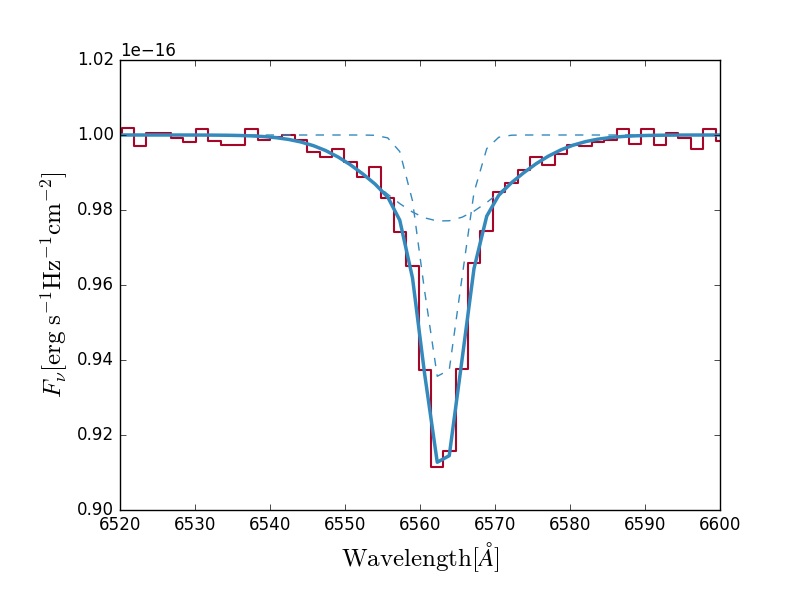
\includegraphics[width=0.7\textwidth]{spectrum.png}
  \label{fig:linea}
  \caption{Las líneas punteadas son las dos gausianas simples cuya suma
    corresponde a la línea azul contínua. La curva roja representa el espectro.
    Como se aprecia, la suma de las dos gausianas simples representa bastante
    bien el espectro (el cual no es originalmente una suma de dos gausianas).
    El mejor fit se obtiene a cambio de un modelo más complejo: esta vez son dos
    gaussianas de centro conocido por lo que el modelo tiene 4 parámetros.}
\end{figure}

Para cada uno de los dos modelos estime, usando métodos Bayesianos, los
parámetros (reporte, por ejemplo, la esperanza $E[\theta]$, de los parámetros),
y sus intervalos de 68\% de confianza, que en estadística Bayesiana se llaman
intervalos de credibilidad.

\begin{ayuda}
  \small
  \noindent {\bf NOTA 1.}

  Ud. deberá definir probabilidades a priori para cada uno de los parámetros de
  los modelos. Sea explícito en su informe sobre cuáles fueron sus elecciones
  y su justificación.

  \vspace{0.5em}
  \noindent {\bf NOTA 2.}

  Para calcular la verosimilitud necesitará los errores asociados a cada punto
  (pixel).  Esta vez asumiremos que los errores son gaussianos y constantes a
  lo largo del espectro. Dado que el contínuo es conocido, Ud. puede estimar el
  \emph{ruido} mirando la variación de los puntos con respecto al valor del
  contínuo conocido. Explicite en su informe el valor que determinó.

\end{ayuda}

\vspace{1em}
\noindent{\large \bf Segunda Parte.}

Como se mencionó antes, el modelo de dos gaussianas debe producir un mejor fit
de los datos, pero a cambio de tener el doble de parámetros libres que el
modelo de una gaussiana simple. Utilice métodos de selección Bayesiana de
modelos para decidir cuál de los dos modelos es una mejor representación de los
datos.  Justifique su decisión.

\begin{ayuda}
  \small
  \noindent {\bf NOTA 1.}

  Ud. deberá realizar una integral en 4 dimensiones en algún momento.  Describa
  claramente el procedimiento que eligió para hacer dicha integral.

\end{ayuda}

\pagebreak
\noindent\textbf{Instrucciones Importantes.}
\begin{itemize}

\item \textbf{NO USE JUPYTER NOTEBOOKS}. Estamos revisando en serio el diseño
  del código por lo que es imprescindible que entregue su código en un archivo
  de texto \texttt{.py}.

\item Evaluaremos su uso correcto de python. Si define una función
  relativametne larga o con muchos parámetros, recuerde escribir el
  \emph{docstring} que describa los parámetros que recibe la función, el
  output, y el detalle de qué es lo que hace la función. Recuerde que
  generalmente es mejor usar varias funciones cortas (que hagan una sola cosa
  bien) que una muy larga (que lo haga todo).  Utilice nombres explicativos
  tanto para las funciones como para las variables de su código. El mejor
  nombre es aquel que permite entender qué hace la función sin tener que leer
  su implementación ni su \emph{docstring}.

\item Su código debe aprobar la guía sintáctica de estilo
  (\href{https://www.python.org/dev/peps/pep-0008/}{\texttt{PEP8}}). Lleva
  puntaje.

\item Utilice \texttt{git} durante el desarrollo de la tarea para mantener un
  historial de los cambios realizados. La siguiente
  \href{https://education.github.com/git-cheat-sheet-education.pdf}{cheat
    sheet} le puede ser útil. {\bf Revisaremos el uso apropiado de la
  herramienta y asignaremos una fracción del puntaje a este ítem.} Realice
  cambios pequeños y guarde su progreso (a través de \emph{commits})
  regularmente. No guarde código que no corre o compila (si lo hace por algún
  motivo deje un mensaje claro que lo indique). Escriba mensajes claros que
  permitan hacerse una idea de lo que se agregó y/o cambió de un
  \texttt{commit} al siguiente.

\item Para hacer un informe completo Ud. debe decidir qué es interesante y
  agregar las figuras correspondientes. No olvide anotar los ejes e incluir una
  \emph{caption} o título que describa el contenido de cada figura. Tampoco
  olvide las unidades asociadas a las cantidades mostradas en los diferentes
  plots (si es que existen).

\item La tarea se entrega subiendo su trabajo a github. Clone este repositorio
  (el que está en su propia cuenta privada), trabaje en el código y en el
  informe y cuando haya terminado asegúrese de hacer un último \texttt{commit}
  y luego un \texttt{push} para subir todo su trabajo a github.

\item El informe debe ser entregado en formato \texttt{pdf}, este debe ser
  claro sin información de más ni de menos. \textbf{Esto es muy importante, no
  escriba de más, esto no mejorará su nota sino que al contrario}. La presente
  tarea probablemente no requiere informes de más de 3 o 4 páginas en total
  (dependiendo de cuántas figuras incluya; esto no es una regla estricta, sólo
  una referencia útil).  Asegúrese de utilizar figuras efectivas y tablas para
  resumir sus resultados. Revise su ortografía.

\end{itemize}


%% FIN ENUNCIADO ===============================================================
%% =============================================================================

\end{document}
